%!TEX root = ../template.tex

\section{Human Body Modelling}

We propose a human body reference model as an articulated multi-body skeleton with rigid
 bodies connected by 3 Degrees-of-Freedom (DoF) joints. Kinematic and dynamic properties 
 are defined as follows.
%
%%%%%%%%%%%%%%%%%%%%%%%%%%%%%%%%%%%%%%%%%%%%%%%%%%%%%%%%%%%%%%%%%%%%%%%%%%%%%%%%%%%%%%%%%%%%%%%%
\subsection{Kinematic properties}
Inspired by the biomechanical model developed for the Xsens MVN motion capture system
 \cite{Roetenberg2009} shown in Fig. \ref{fig:human_models}b, our model consists of a set of 
 23 rigid bodies with simple geometric
  shapes (parallelepiped, cylinder, sphere).  The origin of each link is located at 
  the parent joint origin, (i.e., the joint that connects the link to its
  parent). Figure \ref{fig:figs_human_JointLink}b shows  links and joints of the model.  
  The dimension of 
   each link is estimated by using data coming from motion capture acquisition.
%
\begin{figure}
  \centering
    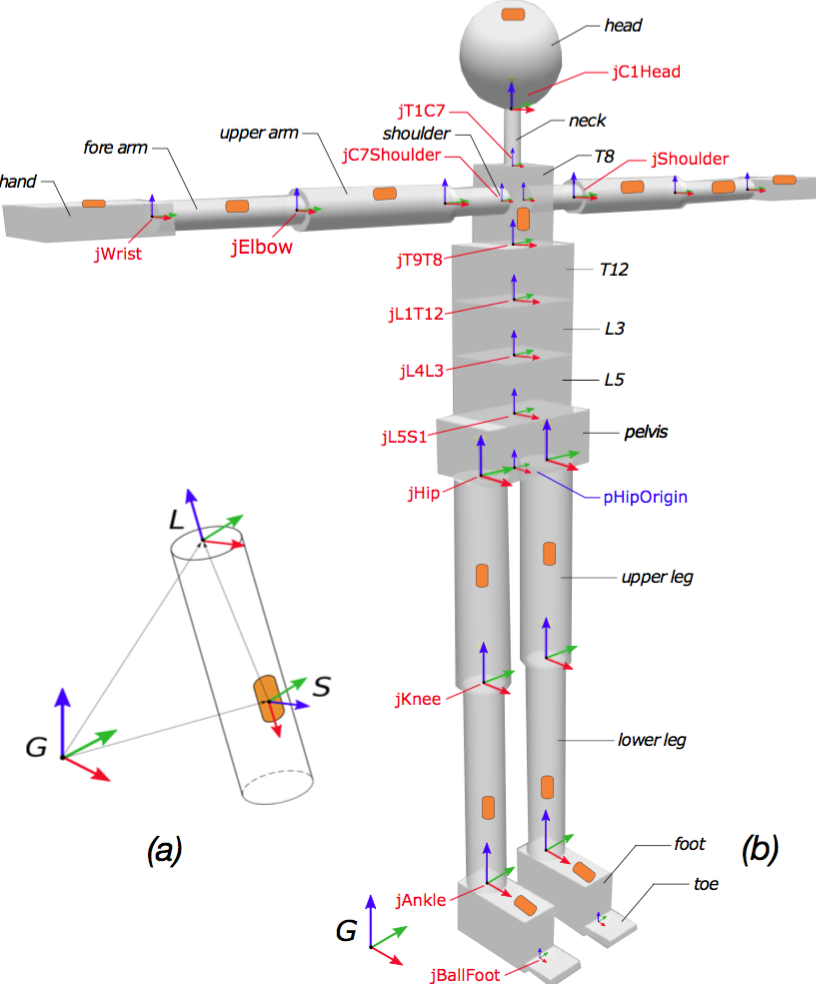
\includegraphics[width=1\columnwidth]{figs/human_JointLink}
\caption[Caption for LOF]{(a) Sensor attached to a generic link. 
(b) Human body reference model with labels for links and joints 
and with sensors distributed in the Xsens suit.  
 Reference frames are also shown\footnotemark.}
  \label{fig:figs_human_JointLink}
\end{figure}
%
\footnotetext{The RGB (Red-Green-Blue) convention for
${x}$-${y}$-${z}$ axes is adopted throughout the paper.}
%
%%%%%%%%%%%%%%%%%%%%%%%%%%%%%%%%%%%%%%%%%%%%%%%%%%%%%%%%%%%%%%%%%%%%%%%%%%%%%%%%%%%%%%%%%%%%%%%%
\subsection{Dynamic properties}
The dynamic properties, such as center of mass and inertia tensor for each link, are not
 embedded in the Xsens output data since they are usually computed in a post-processing phase.
   Since our aim is to have a real-time estimation for the human dynamic variables,
    the knowledge of
    dynamic properties during the acquisition phase is mandatory \cite{Drillis1964}.  Since it is impractical to retrieve these quantities in-vivo for humans, we relied on the
	 available anthropometric data in literature (\cite{Winter1990}, \cite{Herman2007})
	  starting from the total body mass of the
 subject, under the assumptions of geometric approximation and of homogeneous density for
  the rigid bodies (\cite{Hanavan1964}, \cite{Yeadon1990}).  
 %  
%%%%%%%%%%%%%%%%%%%%%%%%%%%%%%%%%%%%%%%%%%%%%%%%%%%%%%%%%%%%%%%%%%%%%%%%%%%%%%%%%%%%%%%%%%%%%%%%
%  \subsection{Sensor position}
% In order to build the model, the information of the position of the sensors for each link is
%  needed. Since it is not provided by Xsens, we exploited the linear acceleration $\bm a$ and
%   the angular velocity $\bm \omega$ measured by sensors in the following way:
%
% \begin{eqnarray} \label{eq:sensorPosEq} \nonumber
% {}^{S} \bm a_{S} &=& {}^{S} \bm R_G \Big( {}^{G} \bm a_{S} - {}^{G} \bm a_g \Big) =\\\nonumber
%                  &=& {}^{S} \bm R_G \Big[ {}^{G} \bm a_{L} + {}^{G} \bm{\dot \omega}_{L}
% 				     \times {}^{G} \bm R_{L} {}^{L} \bm p_{S, L}+\\
%                 &{}& {}^{G} \bm \omega_{L} \times \Big( {}^{G} \bm \omega_{L} \times
% 				     {}^{G} \bm R_{L} {}^{L} \bm p_{S, L}\Big) - {}^{G} \bm a_g \Big],
% \end{eqnarray}
% where $S$ is the frame of the sensor and $L$ is the frame related to the link on which it is
% attached (as in Fig. \ref{fig:figs_human_JointLink}a). By exploiting \eqref{eq:sensorPosEq}
% it is possible to retrieve the position of sensor on the link in
% the link frame ${}^{L} \bm p_{S, L}$.